%%==================================================================%%
%% Author : Tejedo Gonz�lez, Daniel                                 %%
%%          S�nchez Barreiro, Pablo                                 %%
%% Version: 1.0, 25/11/2012                                         %%                   %%                                                                  %%
%% Memoria del Proyecto Fin de Carrera                              %%
%% Sintaxis abstracta, archivo ra�z                                       %%
%%==================================================================%%

\chapterheader{Creaci�n de la sintaxis abstracta}{Creaci�n de la sintaxis abstracta}
\label{chap:metamodelo}

A partir de aqu�, los siguientes cap�tulos tratan de describir en detalle cada una de las tareas expuestas en la planificaci�n del proyecto. Evidentemente, se ha obviado la tarea de documentaci�n, pues no requiere explicaci�n alguna. Este cap�tulo en concreto versa sobre la creaci�n de la sintaxis abstracta del lenguaje, as� como cada una de las subtareas subyacentes.

\chaptertoc

\section{Captura de requisitos}
\label{sec:meta:requisitos}
%%==================================================================%%
%% Author : Tejedo Gonz�lez, Daniel                                 %%
%%          S�nchez Barreiro, Pablo                                 %%
%% Version: 1.0, 25/11/2012                                         %%
%% Version: 2.0, 06/02/2013                                         %%
%%                                                                  %%
%% Memoria del Proyecto Fin de Carrera                              %%
%% Sintaxis abstracta, requisitos                                   %%
%%==================================================================%%

El primer paso para desarrollar nuestro lenguaje era conocer qu� aspecto deb�a tener nuestro lenguaje y qu� restricciones deb�a satisfacer. Es decir, en primer lugar debemos realizar un proceso que podemos denominar de captura de requisitos para poder comprender qu� es lo que tiene que hacer exactamente el lenguaje que se pretende crear.

Concretamente nuestro lenguaje hab�a sido pr�cticamente definido por el profesor Pablo S�nchez, del Departamento de Matem�ticas, Estad�stica y Computaci�n de la Universidad de Cantabria, mediante notaci�n BNF. Las ideas subyacentes a dicho lenguaje son las que se describen a continuaci�n.

%%==================================================================%%
%% NOTA(Pablo): Aqu� traduce la secci�n III del art�culo que te
%%              env�o adjunto. Si te hacen falta las fuentes del
%%              art�culo, me las pides.
%%
%%              Traduce primero del ingl�s y luego lo repasas y lo
%%              reescribes para que suene a castellano
%% 
%%              Si en la secci�n III no aparecen las razones por 
%%              las cuales una caracter�stica es clonable, buscar 
%%              en qu� parte del art�culo aparecen y explicarlo

%%==================================================================%%

Adem�s nuestro lenguaje deb�a permitir vincular un un modelo de caracter�sticas sobre el cual se definir�n un conjunto de restricciones externas. Este modelo se utilizar�, por ejemplo, para comprobar que los s�mbolos que aparecen como nombres de caracter�sticas en las restricciones se refieren a caracter�sticas que realmente existen en el �rbol de caracter�sticas. Por ejemplo, una restricci�n del tipo $AdvancedHeating => Heating$ carecer�a de sentido si algunas de las caracter�sticas $AdvancedHeating$ o $Heating$ no apareciesen en el �rbol de caracter�sticas sobre el cual estamos definiendo restricciones.

%%======================================================================================%%
%% NOTA(Pablo): Esto posiblemente sobre al introducir la traducci�n de la Secci�n III.
%%              Si es as�, eliminarla.
%%              Si los conceptos de restricci�n con contexto y operaci�n cuantificada
%%              no apareciesen, meter esta clasificaci�n pero resumida
%%======================================================================================%%
%%
%% De entre todos esos requisitos b�sicos, es necesario entrar en detalle en el n�mero 3
%% y enumerar la lista de operaciones que pueden ser definidas por nuestro lenguaje. Se
%% pueden clasificar en los siguientes tipos: \\
%%
%% - L�gicas: Son operaciones cuyos operandos han de ser caracter�sticas sin
%%   cardinalidad (tambi�n llamadas caracter�sticas simples), y que se evaluan a
%%   verdadero o falso. Entre las operaciones l�gicas encontramos las cl�sicas not,
%%   and, or, xor e implica.
%%
%% - Num�ricas: Sus operandos han de ser caracter�sticas con cardinalidad (tambi�n
%%   llamadas caracter�sticas m�ltiples) o simplemente n�meros. Su resultado se evalua
%%   con un valor num�rico. Las operaciones num�ricas a implementar son la suma, resta,
%%   multiplicaci�n y divisi�n.
%%
%% - Comparativas: Sus operandos han de ser caracter�sticas m�ltiples o simplemente n�meros,
%%   pero su resultado se evalua con un valor booleano. Las operaciones de comparaci�n a
%%   implementar son igual que, mayor que, menor que, distinto que, mayor o igual que y menor
%%   o igual que.
%%
%% - Operaci�n de contexto: Operaci�n que permite hacer referencia a una caracter�stica
%%   hija de otra caracter�stica. Esta operaci�n tiene sentido para seleccionar
%%   caracter�sticas cuyo nombre pueda estar repetido pero que tengan contextos diferentes.
%%   Por ejemplo, en el modelo de caracter�sticas SmartHome de la figura \ref{figsmarthome}
%%   podemos observar que la caracter�stica HeaterMng est� presente en muchos contextos
%%   diferentes. Esta operaci�n es necesaria para poder saber con seguridad a cual de esos
%%   contextos estamos aplicando la restricci�n.
%%
%% - Operaci�n de selecci�n: Operaci�n que corresponde a los operadores l�gicos cl�sicos
%%   "para todo" o "existe", y que tiene la misma funcionalidad. Evalua si una restricci�n
%%   se cumple para todos los casos en que puede existir  o si se cumple en alguno de los
%%   casos. Por ejemplo, en el modelo de la figura \ref{figsmarthome} se podr�a evaluar una
%%   restricci�n para cada una de las habitaciones que hayan sido definidas, y saber si se
%%  cumple en todas, en alguna o en ninguna.
%%
%%======================================================================================%%

Utilizando esta informaci�n como base, procedimos a crear el correspondiente metamodelo en Ecore para nuestro lenguaje.




\section{Creaci�n del metamodelo}
\label{sec:meta:creacion}
%%==================================================================%%
%% Author : Tejedo Gonz�lez, Daniel                                 %%
%%          S�nchez Barreiro, Pablo                                 %%
%% Version: 1.0, 25/11/2012                                         %%                   %%                                                                  %%
%% Memoria del Proyecto Fin de Carrera                              %%
%% Sintaxis abstracta, creacion metamodelo                                      %%
%%==================================================================%%

Una vez hemos definido cuales son los requisitos del lenguaje, tenemos que construir nuestro metamodelo de tal modo que se ajuste a ellos y sea capaz de cumplirlos. El requisito m�s complejo y que requerir� m�s desaf�os de dise�o es, evidentemente, el de implementar todas las operaciones. As� que empezaremos primero por las partes m�s f�ciles.

Todas las restricciones que sean definidas en cada sintaxis concreta han de ser aplicadas al mismo modelo de caracter�sticas (aunque a varias configuraciones si as� lo desea el usuario). Por lo tanto, la informaci�n relativa al modelo de caracter�sticas sobre el que queremos aplicar esas restricciones es susceptible de ser almacenada en el metamodelo de nuestro lenguaje. Se entiende que el modelo de caracter�sticas que hay que guardar habr� sido previamente creado usando la herramienta Hydra, pues este editor es una extensi�n de la misma. Eso reduce mucho el n�mero de factores de los que hay preocuparse, vi�ndose reducidos en este punto a tener que almacenar �nicamente la localizaci�n del fichero dentro del sistema, para luego poder cargarlo en partes de validaci�n posteriores.

As� pues, nuestra clase inicial Model, que representa el modelo sobre el que aplicaremos las restricciones, tiene un atributo featureList en el que se guardar� la direcci�n del fichero del modelo de caracter�sticas Hydra.

Para permitir que sobre ese modelo que ya hemos representado se puedan definir un n�mero indeterminado de restricciones, es necesario crear una clase Constraint, y relacionar la clase Model con ella. La relaci�n resultante se podr�a expresar como "un modelo tiene de 0 a x restricciones", donde x es cualqueir n�mero entero positivo. 

El requisito correspondiente a la validaci�n de las restricciones que hayamos definido no tiene modo de ser resuelto a estas alturas del desarrollo de nuestra aplicaci�n, por lo que �nicamente queda la implementaci�n de las operaciones. L�gicamente, esta es la tarea de mayor complejidad de nuestro sistema. 

El primer paso es definir toda la estructura necesaria para la implementaci�n de las operaciones, haciendo que cada una de ellas est� representada en nuestro metamodelo mediante una clase, pero sin preocuparnos todav�a por las relaciones entre ellas. La clase ra�z de toda esta estructura es Operand. Es una clase abstracta, es decir, en los modelos que luego instanciemos de este metamodelo no podr� haber ninguna instancia de Operand, s�lo de los hijos no abstractos que tenga. A medida que vayamos definiendo clases hijas  de Operand estaremos especificando cada vez con m�s exactitud a qu� tipo de operaci�n estamos haciendo referencia.

En el segundo nivel de la estructura de implementaci�n de las operaciones hacemos una ramificaci�n seg�n el tipo del valor de retorno o de evaluaci�n de las posibilidades. Es decir, a la clase Operand le a�adiremos dos hijos: BoolOperand para operaciones que se eval�an a booleano y NumOperand para operaciones que se eval�an a num�rico. Estas clases tambi�n ser�n abstractas.

\begin{figure}[t]
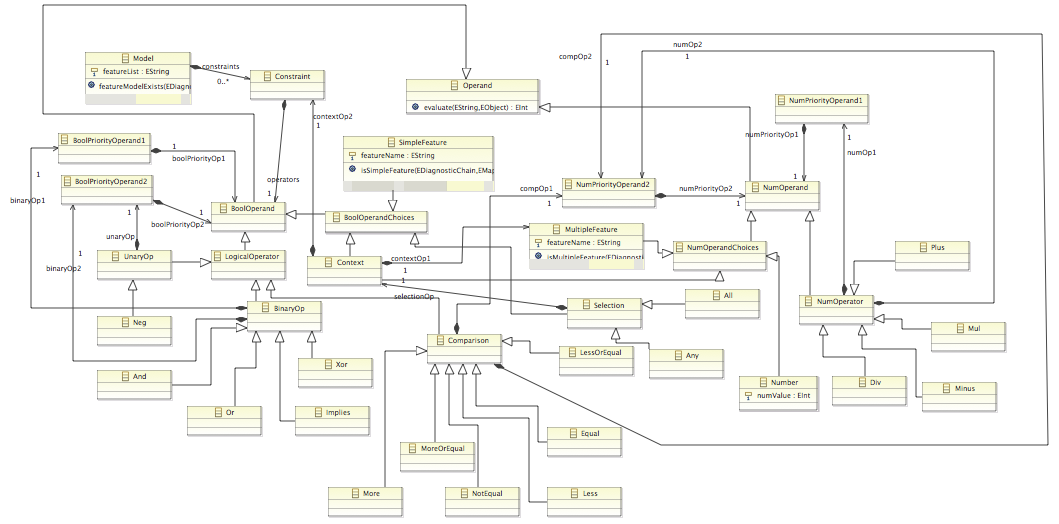
\includegraphics[scale=0.4]{metamodelo/metamodelo.jpg}
\caption{Metamodelo utilizado para la creaci�n de nuestro lenguaje de especificaci�n y validaci�n de restricciones}
\label{figmetameta}
\end{figure}


El proceso de divisi�n a partir de aqu� es m�s o menos an�logo para todas las operaciones, as� que vamos a centrarnos �nicamente en la rama que da lugar a las operaciones binarias l�gicas, para comentar despu�s los casos y situaciones especiales. Una vez tenemos la clase BoolOperand, podemos especializarla un poco m�s a LogicalOperator, que a su vez se dividir� en operaciones unarias, binarias, o de comparaci�n. Todas ellas son clases abstractas. Por fin, la clase BinaryOp heredar� las clases de las operaciones propiamente dichas, en este caso And, Or, Implies y Xor. Estas ya podr�n ser instanciadas en las sintaxis concretas que creemos.

Cabe hacer menci�n tambi�n a las clases SimpleFeature, MultipleFeature y Number, que representan a las caracter�sticas simples, m�ltiples y n�meros respectivamente. En cualquier �rbol resultante de parsear nuestro lenguaje, estas clases representar�n las hojas. En �ltima instancia todas las operaciones tendr�n como operandos caracter�sticas o n�meros. Podemos observar que SimpleFeature es un operando booleano (est� en la parte estructural de las operaciones booleanas) ya que su evaluaci�n ser� verdadero o falso, dependiendo si esa caracter�stica ha sido seleccionada en la configuraci�n correspondiente o no. MultipleFeature sin embargo se eval�a a n�mero entero. Su valor ser� el n�mero de apariciones de esa caracter�stica dentro de la configuraci�n correspondiente.

Muchas de las clases que ahora se pueden contemplar en el metamodelo de la figura \ref{figmetameta} a�n no estaban presentes en esta etapa temprana del dise�o, y su inclusi�n fue necesaria a ra�z de la creaci�n de la gram�tica y los problemas que se observaron en ese punto. En particular, las terminadas en Choices y en PriorityOperand. Las operaciones All, Any y Context en este momento eran simples herencias de BoolOperand. El motivo de estas modificaciones ser� explicado en el cap�tulo siguiente. 

Para terminar este apartado, vamos a hablar de las relaciones entre las diferentes clases de nuestro metamodelo. En este punto del dise�o no eran las mismas que las de la figura \ref{figmetameta} por los motivos explicados anteriormente. Simplemente busc�bamos una forma de relacionar cada operaci�n con los tipos de sus operandos (que tambi�n pueden ser operaciones, como es l�gico). Las operaciones l�gicas binarias tendr�n dos operandos que tambi�n ser�n binarios. En este momento del dise�o binaryOp1 y binaryOp2 iban relacionados a BoolOperand. Del mismo modo que unaryOp. Del mismo modo, compOp1, compOp2, numOp1 y numOp2 (es decir, los operandos de operaciones de comparaci�n y num�ricas respectivamente) estaban relacionados con la clase NumOperand.

La relaci�n de toda estructura de operaciones con los dos elementos anteriores, Model y Constraint, se realiza entre Constraint y BoolOperand. Toda restricci�n en �ltima ha de ser evaluada a verdadero o falso, es por eso que la relaci�n no va con Operand, como podr�a pensarse en primera instancia. De este modo estamos forzando que la operaci�n con menos profundidad del �rbol parseado de nuestra restricci�n sea booleana, y que por lo tanto el resultado final de validar la restricci�n sea un dato booleano. 

Quiz�s a alguien le pueda sorprender el hecho de que la relaci�n "operators" entre Constrain y BoolOperand sea 1..1 y no 1..*. El motivo es que como los operadores de esa primera operaci�n booleana que estamos forzando pueden ser a su vez operaciones, la complejidad en la restricci�n que podemos definir se propaga por ah� en lugar de por la relaci�n creada.







\section{Pruebas del metamodelo}
\label{sec:meta:pruebas}
%%==================================================================%%
%% Author : Tejedo Gonz�lez, Daniel                                 %%
%%          S�nchez Barreiro, Pablo                                 %%
%% Version: 1.0, 27/11/2012                                         %%                   %%                                                                  %%
%% Memoria del Proyecto Fin de Carrera                              %%
%% Gram�tica, pruebas                                       %%
%%==================================================================%%

\begin{figure}[t]
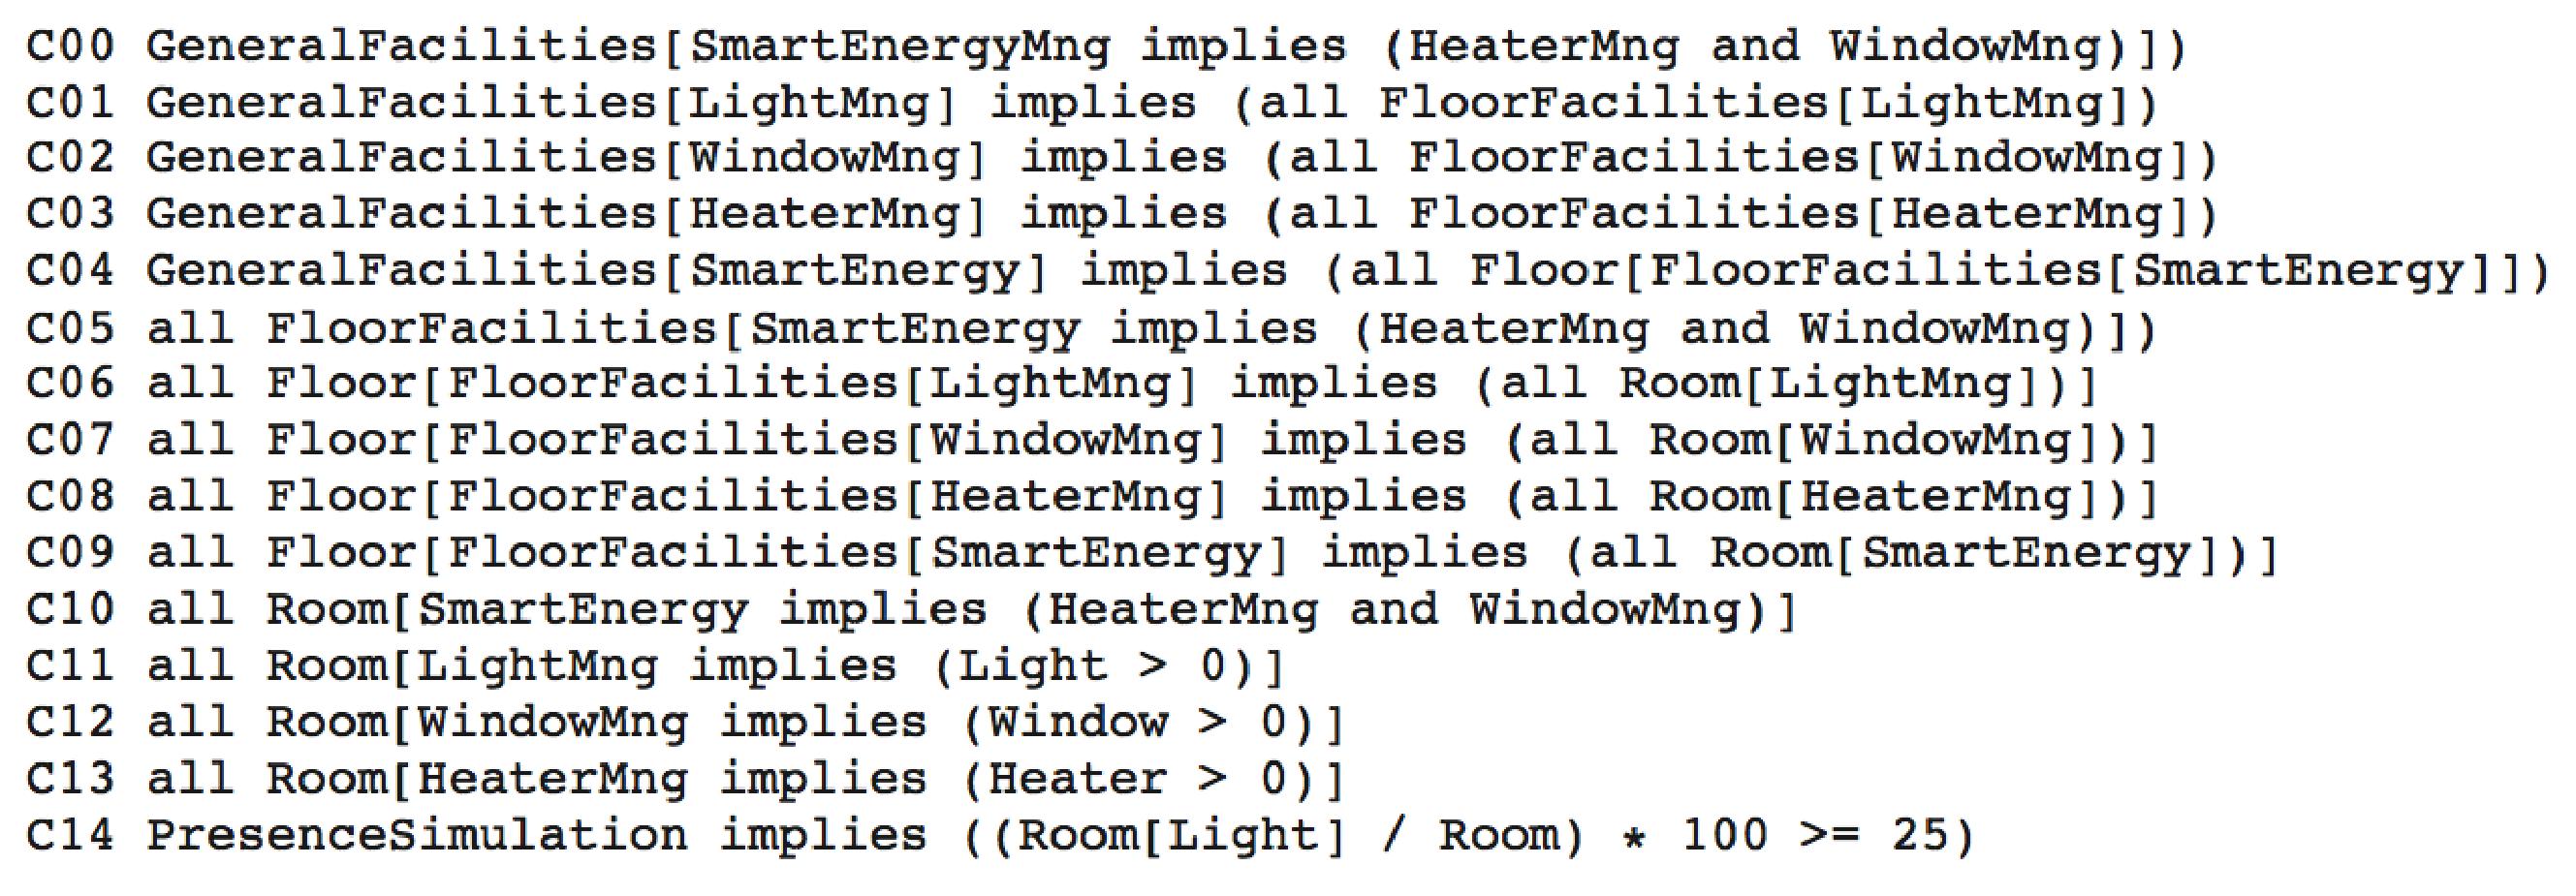
\includegraphics[scale=0.5]{gramatica/oppruebas.eps}
\caption{Bater�a de instrucciones para probar el funcionamiento de la gram�tica}
\label{figgrampruebas}
\end{figure}

Para hacer las pruebas correspondientes a la gram�tica fue de mucha utilidad la vista Outline de Eclipse, que permite obsevar el �rbol de parsing de todos los ficheros de c�digo que creemos en nuestro lenguaje. 

La bater�a de pruebas simplemente consisti� en comprobar una serie de instrucciones y observar dentro de la vista Outline si se parseaban de modo correcto. En este caso se utilizaron unas restricciones definidas en un documento previo de Hydra que conten�an todos los aspectos problem�ticos de la gram�tica, es decir, operaciones largas con prioridad y multitud de contextos. Estas instrucciones son las que se muestran en la figura \ref{figgrampruebas}. 

El resto de operaciones fueron puestas a prueba con restricciones m�s sencillitas y, como en el caso anterior, fueron exitosas. Tambi�n se usaron las instrucciones de las pruebas del cap�tulo anterior, que se pueden observar en la figura \ref{figmetains} para comprobar que el �rbol era el mismo que se cre� en ese momento.
